\section{Bestimmung der Elementarladung nach Millikan} 

\subsection{Vorbereitende Überlegungen}

Zur Vorbereitung dieses Versuches sollte eine Reihe von Aufgaben durchgeführt werden. 
Die Bearbeitung dieser ist im Folgenden dargestellt:
\vspace{0,5cm}

\noindent \textbf{1. Skizzieren Sie die Kräftegleichgewichte.}
	
	Die Kräftegleichgewichte bei einem ein- bzw. ausgeschalteten Plattenkondensator sind in Abb. \ref{fig:force1} und \ref{fig:force2} dargestellt. 
	\begin{figure}
		\centering
		\begin{subfigure}{\textwidth}
			\centering
			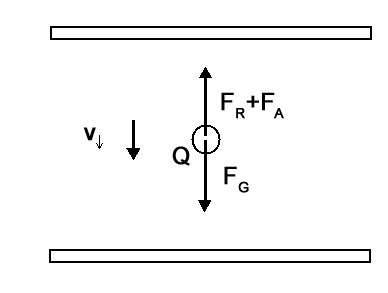
\includegraphics[width=0.5\textwidth]{auswertung/force1.png}
			\caption{Diese Abbildung zeigt das Kräftegleichgewicht bei ausgeschaltetem Kondensator. $F_\text{A}$ ist hierbei die Auftriebskraft, $F_\text{G}$ die Gewichtskraft und $F_\text{R}$ die Reibungskraft, die entgegen der Bewegungsrichtung wirkt\cite{RCL}.}
			\label{fig:force1}
		\end{subfigure}
		\begin{subfigure}{\textwidth}
			\centering
			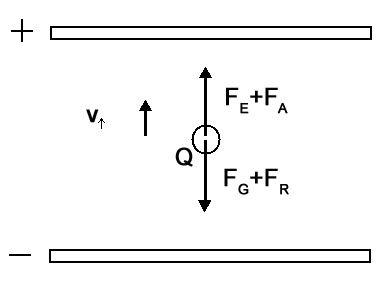
\includegraphics[width=0.5\textwidth]{auswertung/force2.png}
			\caption{Diese Abbildung zeigt das Kräftegleichgewicht bei eingeschaltetem Kondensator. $F_\text{A}$ ist hierbei die Auftriebskraft, $F_\text{G}$ die Gewichtskraft, $F_\text{E}$ die Kraft des elektrischen Feldes, das auf die Ladung des Öltröpfchens wirkt und $F_\text{R}$ die Reibungskraft, die entgegen der Bewegungsrichtung wirkt\cite{RCL}.}
			\label{fig:force2}
		\end{subfigure}
		\caption{Kräftegleichgewichte bei ein- und ausgeschaltetem Plattenkondensator.}
		\label{fig:force}
	\end{figure}
	
\vspace{0,5cm}
\noindent \textbf{2. Leiten Sie aus den Kräftegleichgewichten die Formeln für r und Q her.}

	Für die Kräftegleichgewichte gelten wie in Abb. \ref{fig:force} skizziert:
	\begin{align}
		\label{eq:force1}
		F_\text{G} = F_\text{R} + F_\text{A} \\
		\label{eq:force2}
		\text{und} \quad F_\text{G} + F_\text{R} = F_\text{E} + F_\text{A}.
	\end{align}
	Drückt man das Gewicht $m$ der Öltröpfchen durch ihre Dichte und Volumen\footnote{Dafür wird angenommen, dass die Dichte der Tröpfchen homogen verteilt ist und dass sie kugelförmig mit Radius $r$ sind. Ebenso mit dem Volumen von Luft bei der Auftriebskraft.} aus, sowie dass  so folgt:
	\begin{align}
		\frac{4}{3}\pi r^3 \cdot \rho_\text{Öl} \cdot g = F_\text{G}\\
		\frac{4}{3}\pi r^3 \cdot \rho_\text{Luft} \cdot g = F_\text{A}\\
		6\pi \cdot r \cdot \eta v = F_\text{R} \\
		\frac{U}{d} \cdot Q = F_\text{E}. \label{eq:eForce}
	\end{align}
	Je nach Bewegungsrichtung wird für die Geschwindigkeit $v_{\downarrow}$ bzw. $v_{\uparrow}$ eingesetzt. Für die elektrische Feldkraft wurde die für Plattenkondensatoren bekannte Gleichung verwendet. Das verwendete $\eta$ in der Gleichung für die Reibungskraft entspricht der dynamischen Viskosität der Luft.
	Einsetzen der Kräfte in Gl. \ref{eq:force1} und Gl. \ref{eq:force2} sowie Umformen nach $Q$ bzw. $r$ führt zu:
	\begin{align}
		Q = \frac{18\pi d}{U} \sqrt{\frac{\eta^3 v_\downarrow}{2(\rho_\text{Öl}-\rho_\text{Luft})g}}(v_\downarrow + v_\uparrow) \\
		\text{und} \quad r = 3 \sqrt{\frac{\eta v_\downarrow}{2(\rho_\text{Öl}-\rho_\text{Luft})g}}
	\end{align}
	
\vspace{0,5cm}
\noindent \textbf{3. Schätzen Sie die Dauer der Beschleunigungsphasen nach den Richtungswechseln eines Öltröpfchens mit dem Radius $r = \SI{0,727}{\mu\m}$, indem Sie in beiden Fällen die Gleichung für das Kräftegleichgewicht nach der Geschwindigkeit auflösen und die Beschleunigung abschätzen. Muss die Beschleunigungsphase bei der Zeitmessung berücksichtigt werden?}

	Nein, die Beschleunigungsphase muss nicht berücksichtigt werden, da die erhaltenen Geschwindigkeiten nach dem Einsetzten in einem Bereich von \SI{0,0001}{\meter\per\second} liegen und unter Berücksichtigung der zurückzulegenden Strecke somit keine lange Beschleunigungsphase vorliegen kann.
	
\vspace{0,5cm}
\noindent \textbf{4. Warum ist es wichtig, die Kondenstorplatten waagerecht auszurichten?}

	Es ist wichtig, die Platten waagerecht auszurichten, damit ein homogenes elektrisches Feld entsteht, dessen Feldkraft entgegen der Gewichtskraft verläuft, was im Falle einer nicht waagerechten Ausrichtung nicht möglich ist.

\vspace{0,5cm}
\noindent \textbf{5. Warum sind Öltröpfchen besser geeignet als Wassertröpfchen, wenn man bedenkt, dass die Masse der untersuchten Objekte als konstant angesehen wird?}

	Öl ist verglichen mit Wasser schwerflüchtiger, was bedeutet, dass Öl seine Masse eher behält als Wasser z. B. langsamer verdunstet, was für die längere Betrachtung eines einzelnen Tröpfchens von Vorteil ist.

\vspace{0,5cm}
\noindent \textbf{6. Bewegen sich gering geladene Tröpfchen im elektrischen Feld schneller oder langsamer als stark geladene? Wie ist (qualitativ) dementsprechend die Spannung zu wählen, wenn man gering bzw. stark geladene Öltröpfchen bei etwa gleicher Geschwindigkeit beobachten will?}

	Da die elektrische Feldkraft, wie sie in Gl. \ref{eq:eForce} aufgeführt ist, mit größerer Ladung $Q$ größer wird, bewegen sich stärker geladene Tröpfchen schneller als welche mit geringerer Ladung. Zur Betrachtung gleicher Geschwindigkeiten folgt aus der gleichen Formel, dass eine kleinere Spannung $U$ für stärker geladene Tröpfchen gewählt werden sollte, damit diese sich langsamer bewegen. Umgekehrt müssen höhere Spannung für Tröpfchen geringerer Ladung gewählt werden, insofern diese dieselbe Geschwindigkeit wie stärker geladene Tröpfchen annehmen sollen.

\vspace{0,5cm}
\noindent \textbf{7. Welcher Nachteil ergibt sich für die Auswertung, wenn man die fünf Zeitmessungen mit einer Additionsstoppuhr aufsummiert und durch fünf teilt, anstatt alle fünf Werte zu protokollieren und dann zu mitteln?}

	Bei einer einzelnen Messung ist die Betrachtung der Unsicherheiten zwar einfacher, jedoch muss die ganze Messung für ein Tröpfchen wiederholt werden, sobald die Messung eines Streckenabschnitts zu kurz oder zu lang geraten ist. Für das Aufsummieren kann einfach eine zusätzliche Messung für diesen Streckenabschnitt durchgeführt werden.

\vspace{0,5cm}
\noindent \textbf{8. Wie hängen die Viskosität $\eta$ und die mittlere freie Weglänge $\lambda$ qualitativ von der Temperatur ab?}

	Bei steigender Temperatur erhöhen sich die Viskosität $\eta$ und die mittlere freie Weglänge $\lambda$.\footnote{Dies folgt aus den Literaturwerten, welche der Versuchsanleitung beilagen. Dies gilt jedoch nicht für alle Medien.}
	
\subsection{Methoden}

\subsubsection{Aufbau}

\begin{figure}[ht]
	\centering
	\begin{subfigure}{\textwidth}
		\centering
		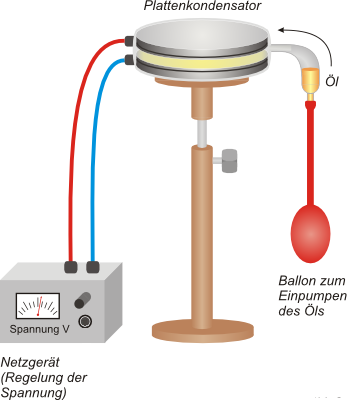
\includegraphics[width=0.5\textwidth]{auswertung/aufbau_1.png}
		\caption{Allgemeine Darstellung des Versuchaufbaus. Zu erkennen ist das Netzgerät mit dem Spannung von bis zu \SI{600}{\volt} für den ebenfalls dargestellten Plattenkondensator, sowie auch die Düse zum Einspritzen des Öls.\cite{Aufbau}}
		\label{fig:aufbau1}	
	\end{subfigure}
	\begin{subfigure}{\textwidth}
		\centering
		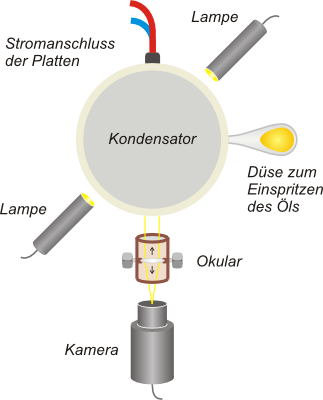
\includegraphics[width=0.45\textwidth]{auswertung/aufbau_2.png}
		\caption{Genauere Darstellung des Aufbaus bezüglich der Betrachtung der Öltröpfchen über das Mikroskop, welches hier aus Kamera und Okular zusammengesetzt ist. Zudem ist die Beleuchtung der Öltröpfchen über die Lampen skizziert.\cite{Aufbau}}
		\label{fig:aufbau2}	
	\end{subfigure}
	\caption{Aufbau des Millikan Versuchs.}
	\label{fig:aufbau}	
\end{figure}

Der Aufbau des Versuches ist in Abb. \ref{fig:aufbau} skizziert. 
Zu erkennen ist der Plattenkondensator, welcher einerseits an ein Netzgerät angeschlossen ist, welches Spannungen von bis zu \SI{600}{\volt} liefern kann, und andererseits an die Düse mit der das Öl in den Plattenkondensator gespritzt wird.
Für die Betrachtung der Öltröpfchen wird ein Mikroskop so an den Plattenkondensator angebracht, dass sich die Tröpfchen in dem Raum zwischen den beiden Platten des Kondensators betrachten lassen. 
Um die Tröpfchen besser zu erkennen wird Licht in den Zwischenraum des Kondensators gestrahlt.
Der Kondensator ist so gepolt, dass das die elektrische Feldkraft der Gewichtskraft entgegenwirkt.

\subsubsection{Unsicherheiten} %TODO richtig?

Die bei diesem Versuch auftretenden Unsicherheiten setzen sich aus der Unsicherheit für die Zeitmessung und der des Ortes zusammen.
Für die Zeitmessung dient eine handelsübliche Stoppuhr.
Diese besitzt eine Digitalanzeige und erhält deswegen eine Unsicherheit, welche über eine Rechteckverteilung bestimmt wird.
Da jedoch auch die Reaktionszeit eine Rolle spielt, wird diese mit \SI{0,1}{\second} über eine Dreiecksverteilung bestimmt.
Aus der kombinierten Unsicherheit der Stoppuhr und der Reaktionszeit folgt die der Zeitmessung.
Bei der Unsicherheit des Ortes wird die des Maßes an dem Mikroskop verwendet.
Hierbei handelt es sich um ein Mikrometermaß, welches eine Unsicherheit von \SI{0,1}{\micro\meter} dreiecksverteilt besitzt.
Die Berechnung der kombinierten Unsicherheiten erfolgt nach GUM und ist im Anhang aufgeführt.

\subsection{Durchführung und Datenanalyse}

Damit sich die Elementarladung der Tröpfchen bestimmen lässt, werden zunächst die Geschwindigkeiten $v_{\downarrow}$ und $v_{\uparrow}$ ermittelt.
Dazu wird die Zeit gemessen, welche das Tröpfchen benötigt um zwei Skalen-abstände auf dem Mikrometermaß an dem Mikroskop zurückzulegen.
Bei ausgeschaltetem Kondensator, wo die Gewichtskraft $F_\text{G}$ auf das Tröpfchen wirkt und dieses sich dadurch nach unten bewegt, wird die gemessene Geschwindigkeit $v_{\downarrow}$ genannt.
Umgekehrt ist $v_{\uparrow}$ die Geschwindigkeit für den Fall, dass der Kondensator eingeschaltet ist und die elektrische Kraft $F_\text{E}$ auf das Tröpfchen wirkt, sodass es sich nach oben bewegt. 

% TODO

\subsection{Diskussion}

% TODO

